\documentclass[tikz]{standalone}
\usepackage{amsmath,mathtools}
\usetikzlibrary{positioning,calc,chains,shapes.multipart}
\begin{document}
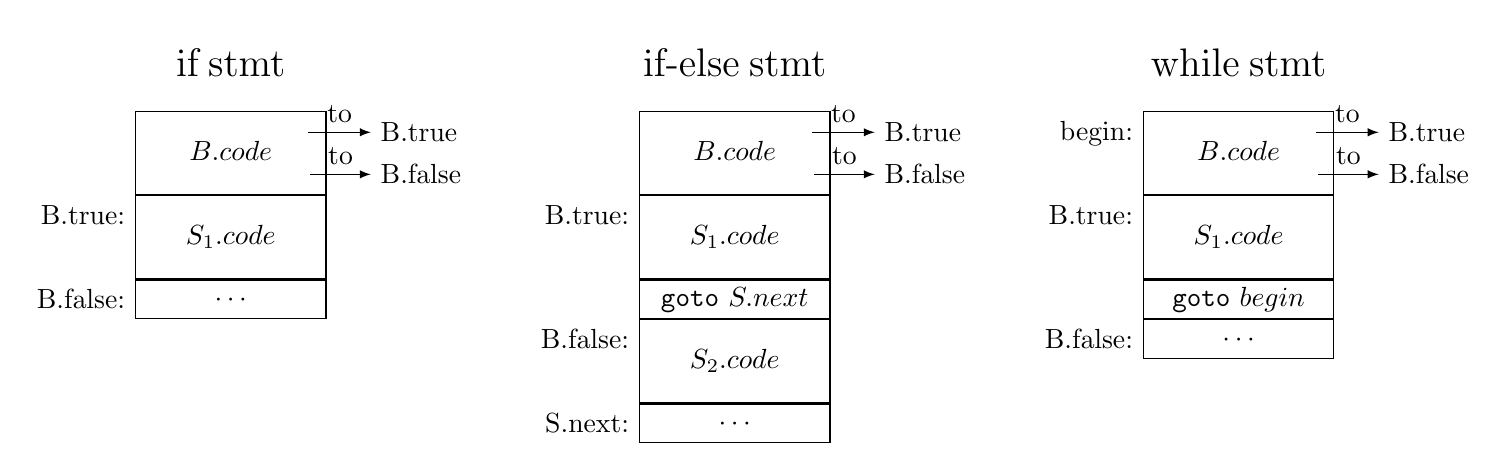
\begin{tikzpicture}[
  node distance = 0ex and 1.5ex,
  simple node/.style={
    draw,
    inner sep=0pt,
    minimum height = 3em,
    text width=16ex,
    text height=2.4ex,
    text depth=1.2ex,
    align=center,
    font=\linespread{.9}\selectfont,
  },
  split node/.style={
    simple node,
    rectangle split,
    rectangle split parts=#1,
    rectangle split ignore empty parts,
    rectangle split part align=base,
    draw,
    inner sep=0ex,
  },
  split horizon node/.style={
    simple node,
    rectangle split,
    rectangle split parts=#1,
    rectangle split ignore empty parts,
    draw,
    inner sep=0ex,
    rectangle split part align=base,
  },
  narrow node/.style={
    simple node,
    minimum height = 1.4em,
    text height=1.2ex,
    text depth=0,
  },
  start chain = going below,
  ]
  {[start chain]
    \coordinate[on chain] (1c1b8a99-a688-4eb2-82bd-a90c53c49e07) at (0,0);
    \node[on chain,simple node,draw=none] {\Large if stmt};
    \node[on chain,simple node] (if-stmt-code) {\(B.code\)};
    \node[on chain,simple node] (if-stmt-true) {\(S_{1}.code\)};
    \node[on chain,narrow node] (if-stmt-false) {\(\cdots\)};
  }
  {[start chain]
    \coordinate[on chain] (e504ee01-0d41-4c77-b56d-52a92e7f9445) at (6.4,0);
    \node[on chain,simple node,draw=none] {\Large if-else stmt};
    \node[on chain,simple node] (if-else-stmt-code) {\(B.code\)};
    \node[on chain,simple node] (if-else-stmt-true) {\(S_{1}.code\)};
    \node[on chain,narrow node] {\(\texttt{goto}\ S.next\)};
    \node[on chain,simple node] (if-else-stmt-false) {\(S_{2}.code\)};
    \node[on chain,narrow node] (if-else-stmt-next) {\(\cdots\)};
  }
  {[start chain]
    \coordinate[on chain] (fa28e31f-4a01-496c-b4d0-e5b7fc6f8f43) at (12.8,0);
    \node[on chain,simple node,draw=none] {\Large while stmt};
    \node[on chain,simple node] (while-stmt-code) {\(B.code\)};
    \node[on chain,simple node] (while-stmt-true) {\(S_{1}.code\)};
    \node[on chain,narrow node] {\(\texttt{goto}\ begin\)};
    \node[on chain,narrow node] (while-stmt-false) {\(\cdots\)};
  }
  \node[left=0 of if-stmt-true.north west,anchor=north east] {B.true:};
  \node[left=0 of if-stmt-false.north west,anchor=north east] {B.false:};
  \node[left=0 of if-else-stmt-true.north west,anchor=north east] {B.true:};
  \node[left=0 of if-else-stmt-false.north west,anchor=north east] {B.false:};
  \node[left=0 of if-else-stmt-next.north west,anchor=north east] {S.next:};
  \node[left=0 of while-stmt-code.north west,anchor=north east] {begin:};
  \node[left=0 of while-stmt-true.north west,anchor=north east] {B.true:};
  \node[left=0 of while-stmt-false.north west,anchor=north east] {B.false:};

  \node[right=1.6em of $(if-stmt-code.east)!0.5!(if-stmt-code.north east)$]
  (if-stmt-to-true) {B.true};
  \node[right=1.6em of $(if-stmt-code.east)!0.5!(if-stmt-code.south east)$]
  (if-stmt-to-false) {B.false};
  \node[right=1.6em of $(if-else-stmt-code.east)!0.5!(if-else-stmt-code.north east)$]
  (if-else-stmt-to-true) {B.true};
  \node[right=1.6em of $(if-else-stmt-code.east)!0.5!(if-else-stmt-code.south east)$]
  (if-else-stmt-to-false) {B.false};
  \node[right=1.6em of $(while-stmt-code.east)!0.5!(while-stmt-code.north east)$]
  (while-stmt-to-true) {B.true};
  \node[right=1.6em of $(while-stmt-code.east)!0.5!(while-stmt-code.south east)$]
  (while-stmt-to-false) {B.false};

  \draw[latex-] (if-stmt-to-true) edge node[above]{to} ++(-4em,0);
  \draw[latex-] (if-stmt-to-false) edge node[above]{to} ++(-4em,0);
  \draw[latex-] (if-else-stmt-to-true) edge node[above]{to} ++(-4em,0);
  \draw[latex-] (if-else-stmt-to-false) edge node[above]{to} ++(-4em,0);
  \draw[latex-] (while-stmt-to-true) edge node[above]{to} ++(-4em,0);
  \draw[latex-] (while-stmt-to-false) edge node[above]{to} ++(-4em,0);
\end{tikzpicture}
\end{document}
